\chapter{Classification based on malware's meta-data using decision tree approach}\label{chap:4}
%EXPERIMENTAL RESULTS AND ANALYSIS
%
%
This chapter describes Win32 executive files structure, known as PE files structure, that is used in classification system as malware meta-data. Afterwards, the machine learning technique called decision tree method is mentioned in classification malware system. Finally, this chapter presents classification based on malware's meta-data using decision tree approach. 

\section{PE file format\cite{peheaderci}}
\subsection{Overview of the PE File Format}

The Portable Executable (PE) file format has been designed for use by all Win32 based system. The general layout of a PE file is given in Figure \ref{fig:pefiles}. As shown in Figure \ref{fig:pefiles} PE header consists of four parts: a MS-DOS session includes DosMZ header and Dos stub; PE header; a section table; and images pages consist of several different regions such as .text session, and .data session.
\begin{figure}[h!]
\centering
\includegraphics[width=0.5\textwidth]{graph/pefiles.png}
\caption{The general layout of a PE file.}
\label{fig:pefiles}
\end{figure}

The PE file format start with DOS MZ header. The first two bytes - "MZ" of the header is the DOS EXE signature. The first few hundred bytes of the typical PE file are taken up by the MS-DOS stub. This stub is a tiny program that displays a string like "This program cannot be run in MS-DOS mode.". 

The following part is PE header. The fields of this structure contain only the most basic information about the file such as the locations and sizes of the code and the data areas. These data structures of PE header will be explained shortly.

Following the PE header is the session table. The section table is an array of IMAGE\_SECTION\_HEADERs structures. An IMAGE\_SECTION\_HEADER provides information about its associated section such as location, length, and characteristics. The number of elements in this array is given in the PE header, known as NumberOfSections field. At a minimum, there are commonly at least two sections in a PE file: code and data. Figure  shows a section table for a typical PE file.

\begin{figure}[h!]
\centering
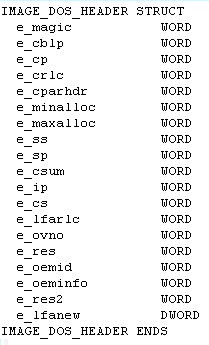
\includegraphics[width=0.5\textwidth]{graph/dosHeaderStructure.png}
\caption{A section table for a typical PE file.}
\label{fig:pefiles}
\end{figure}

That is all about the physical layout of the PE file format. The major steps in loading a PE file into memory is described as follow:

\begin{itemize}
\item When the PE file is running, the PE loader examines the DOS MZ header for the offset of the PE header. If it is found, it would skip to the PE header.
\item The PE loader checks if the PE header is valid. Then, it goes to the end of the PE header if the PE header is valid.
\item Following the PE header is the section table. The PE header reads information about the sections and maps those sections into memory using file mapping. It also gives each section the attributes as specified in the section table.
\item After the PE file is mapped into memory, the PE loader concerns itself with the logical parts of the PE file, such as the import table.
\end{itemize}
\begin{figure}[h!]
\centering
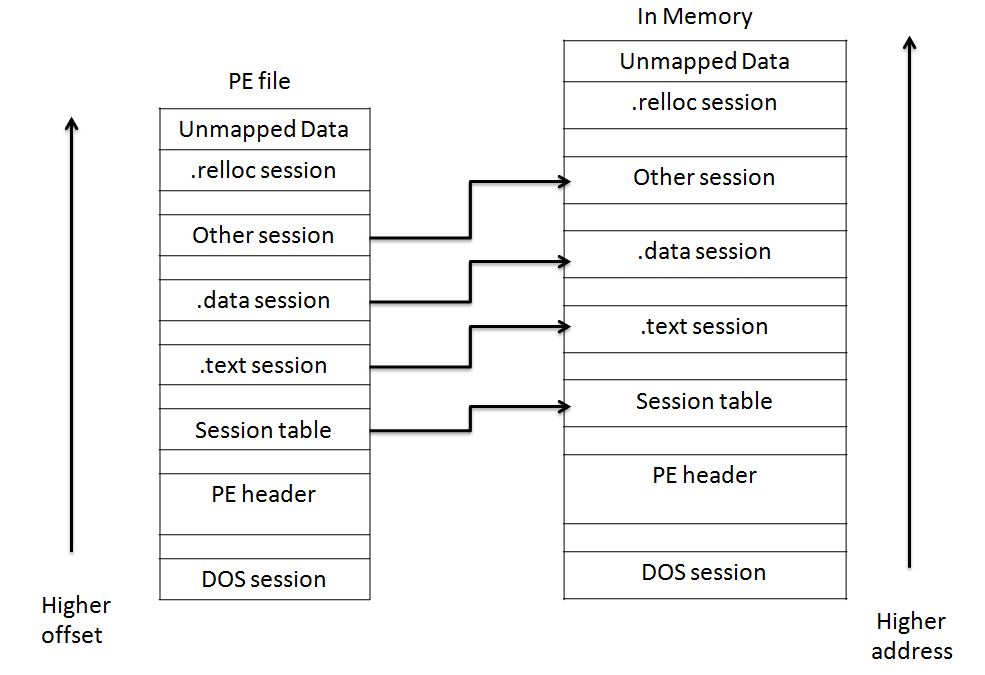
\includegraphics[width=1\textwidth]{graph/pe1.png}
\caption{PE file format.}
\label{fig:pe1}
\end{figure}


\subsection{The PE Header}


\begin{figure}[httb]
\centering
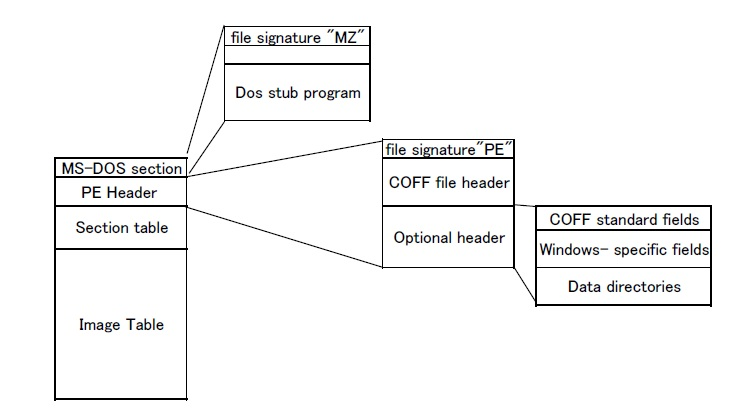
\includegraphics[width=1\textwidth]{graph/peheader1.jpg}
\caption{Layout a file in PE header format.}
\label{fig:peheader}
\end{figure}
The PE header is second part of PE files structure. The PE header starts with two characters "PE" known the PE header file signature. The main PE header is a structure of type IMAGE\_NT\_HEADERS, which is defined in WINNT.H. The structure of PE header consists of a DWORD and two substructures composed of FileHeader and OptionalHeader. IMAGE\_NT\_HEADERS contains the three fields:\\
DWORD Signature;\\
IMAGE\_FILE\_HEADER FileHeader;\\
IMAGE\_OPTIONAL\_HEADER OptionalHeader;

Following the PE signature DWORD in the PE header is a structure of type IMAGE\_FILE\_HEADER. The fields of this structure contain only the most basic information about the file. The fields of the IMAGE\_FILE\_HEADER includes:
\begin{itemize}
\item WORD Machine: The CPU that this file is intended for.
\item DWORD NumberOfSections: The number of the members in section
\item DWORD TimeDateStamp: The time that the linker
\item DWORD PointerToSymbolTable: The file offset of the COFF symbol table. 
\item WORD NumberOfSymbols: The number of symbols in the COFF symbol table.
\item WORD SizeOfOptionalHeader: The size of an optional header that can follow this structure.
\item WORD Characteristics: The size of an optional header that can follow this structure. If there are no relocations in this file, characteristics will be 0x0001. If there are no relocations in this file, characteristics will be 0x0001 . If file is an executable image, characteristics will be 0x0002.  If file is a dynamic-link library, not a program, characteristics will be 0x2000.
\end{itemize}



Following the file header is the Optional header which consists of three parts. The first part includes the COFF standard field which contains the sizes of various parts of code, and the \emph{AddressOfEntryPoint} which indicates the location of the entry point of the application and the location of the end of the Import Address Table(IAT).
The fields of Optional header are described as follow: 
\begin{itemize}
\item WORD Magic: appears to be set to 0x010B.
\item BYTE MajorLinkerVersion
\item BYTE MinorLinkerVersion: the version of the linker that produced this file.
\item DWORD SizeOfCode: this field matches the size of the .text section.
\item DWORD SizeOfInitializedData: 
\item DWORD SizeOfUninitializedData: 
\item DWORD AddressOfEntryPoint: 
\item DWORD BaseOfCode: 
\item DWORD BaseOfData: 
\item DWORD ImageBase: 
\item DWORD SectionAlignment: 
\item DWORD FileAlignment: 
\item WORD MajorOperatingSystemVersion: 
\item WORD MinorOperatingSystemVersion: 
\item WORD MajorImageVersion: 
\item WORD MinorImageVersion: 
\item WORD MajorSubsystemVersion: 
\item WORD MinorSubsystemVersion: 
\item DWORD Reserved1: 
\item DWORD SizeOfImage: 
\item DWORD SizeOfHeaders: 
\item DWORD CheckSum: 
\item WORD Subsystem: 
\item WORD DllCharacteristics: 
\item DWORD SizeOfStackReserve:
\item DWORD SizeOfStackCommit: 
\item DWORD SizeOfHeapReserve:
\item DWORD SizeOfHeapCommit: 
\item DWORD LoaderFlags: 
\item DWORD NumberOfRvaAndSizes:
\item IMAGE\_DATA\_DIRECTORY DataDirectory:
\end{itemize}

\section{Decision tree\cite{wikipedia}}
Decision tree is a algorithm generally used in machine learning technique. Decision tree is to create a model that predicts the value of a target variable based on several input variables. An example is shown on the right. Each interior node corresponds to one of the input variables; there are edges to children for each of the possible values of that input variable. Each leaf represents a value of the target variable given the values of the input variables represented by the path from the root to the leaf.

In data mining, trees can be described also as the combination of mathematical and computational techniques to aid the description, categorization and generalization of a given set of data.
Data comes in records of the form
\(\textbf{x},Y\) = \(x_1, x_2, x_3, ..., x_k, Y\)
The dependent variable, Y, is the target variable is analysed to understand, classify or generalise. The vector x is composed of the input variables, x1, x2, x3, that are used for that task.
\section{Classification based on malware's meta-data using decision tree approach}
To make malware classification rapid and correct, decision tree algorithm is used in malware classification system.

As the previous section, Data comes in records of the form:
\(\textbf{x},Y\) = \(x_1, x_2, x_3, ..., x_k, Y\)
In malware classification system, Y is malware families name, \(x_1, x_2, x_3, ..., x_k, Y\) is meta-data. Malware name is provided by anti-virus engines that presented in chapter \ref{chap:2} cannot used in this system. The new malware families is required for detect meaningful characterization of malware. This classification system use famous malware families that reported in Information technology agency such as netsky, mydoom, autorun, mytob, and other famous malware families. Therefore, when new malware is classified into famous malware families, researcher detect some meaningful characterize of malware, and reduce time for malware analysis. 

